\section{Пример 2: построение кривой по данным}

В этом примере мы будем оценивать функцию регрессии двумя способами, сначала с помощью стандартного метода наименьших квадратов, а затем с помощью современного метода построения кривой по данным, который называется \textit{loess}. Мы начнём с краткого повторения теории регрессии. В главе 9 снова рассматривается задача регрессии и дан альтернативный бутстреп метод для оценки стандартных ошибок регрессии. На рисунке 7.5 показан типичный набор данных, для которого используются регрессионные методы:  мужчин приняли участие в эксперименте, чтобы определить, уменьшает ли лекарство на основе холостирамина уровень холестерина в крови. Мужчины должны были принимать по 6 пакетиков холостирамина в день, однако многие из них принимали гораздо меньше.
\\~\\
\noindent
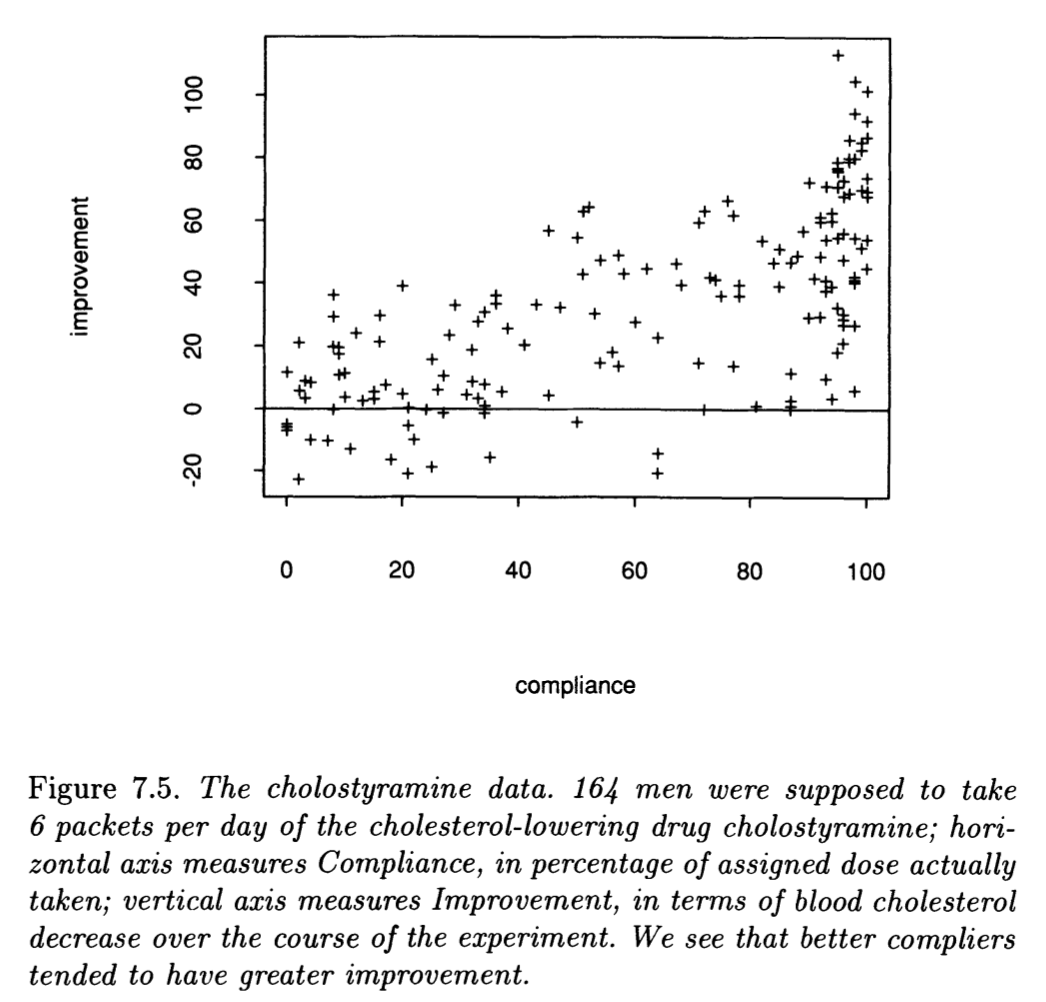
\includegraphics[width=0.9\linewidth]{6/f75.png}
\newline
\setcounter{figure}{1}

Горизонтальная ось, которую мы назовём <<$z$>>, измеряет <<Соответствие>>, то есть процент приёма от назначенной дозы,
$$
z_i = \text{ процент соответствия для мужчины } i,\, i = 1,2,\ldots, 164.
$$

Соответствие измерялось подсчётом количества пакетиков, которые вернули индивиды. Те, кто приняли все пакетики, находятся в правом краю графика; те, кто не принимал ничего --- в левом. Горизонтальная ось, отмеченная <<$y$>>, есть показатель \textit{Улучшения}, уменьшение уровня холестерина в кровяной плазме за время исследования,
$$
y_i = \text{ уменьшение уроня холестерина в крови для индивида } i,\, i = 1,2,\ldots, 164.
$$
Полный набор данных представлен в таблице 7.4.
\\~\\
\noindent
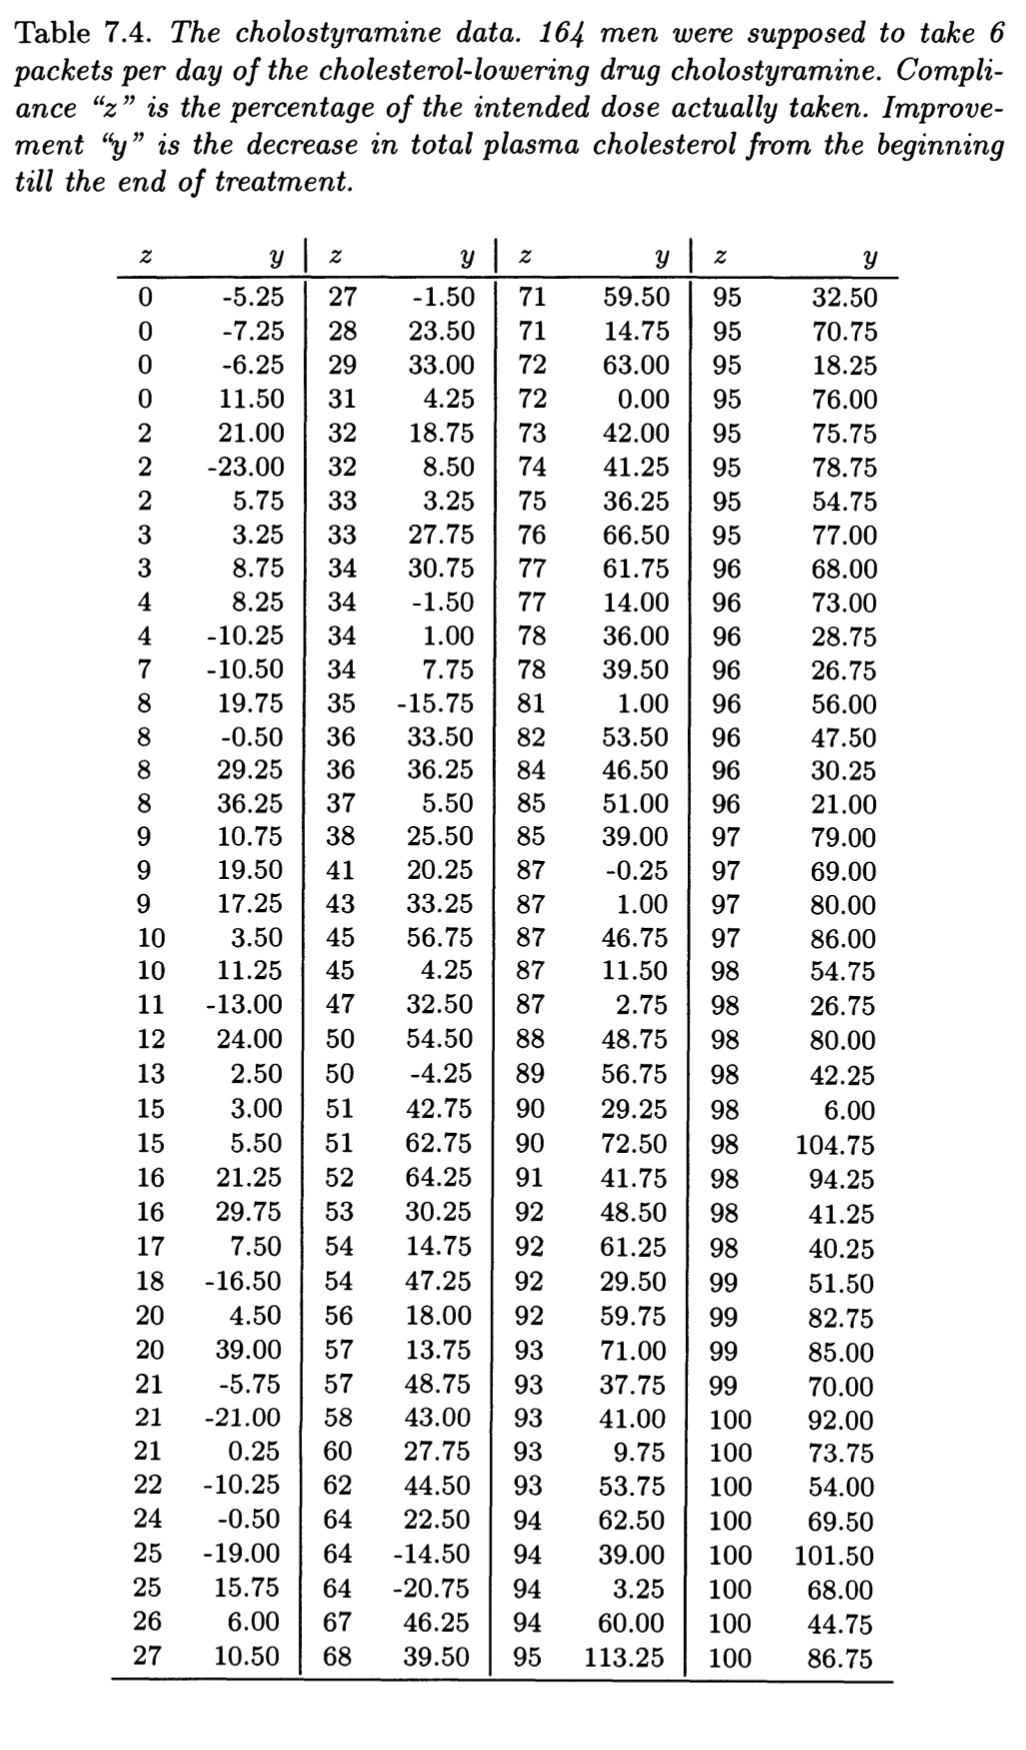
\includegraphics[width=0.95\linewidth]{6/t74.png}
\newline
\setcounter{table}{4}

 На рисунке видно, что мужчины, которые принимали больше хлоростирамина, в целом улучшили свои показатели холестерина, что и ожидалось. То, что мы видим на рисунке 7.5, или скорее то, что мы хотели бы видеть, есть увеличение среднего ответа $y$ в то время как $z$ увеличивается от 0 до $100\%$. На рисунке 7.6 показаны данные вместе с двумя графиками,
\begin{equation}
\hat r_\text{quad}(z) \text{ и }  \hat r_\text{loess}(z).
\end{equation}
\\~\\
\noindent
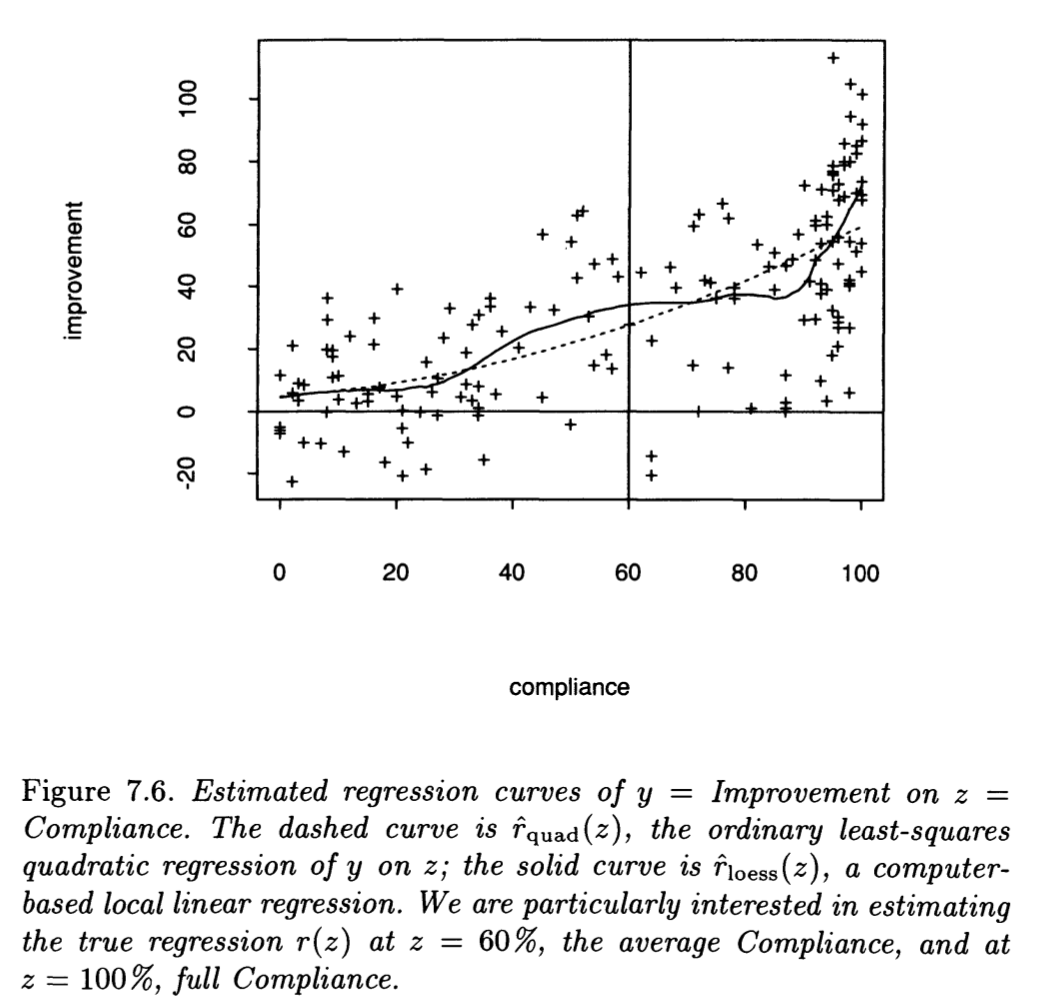
\includegraphics[width=0.9\linewidth]{6/f76.png}
\newline
\setcounter{figure}{7}

Каждый из них есть оценка кривой регрессии. Сейчас будет краткое повторение построения и оценки регрессионных кривых.
По определению регрессией ответа $y$ на независимую переменную $z$ называется условное математическое ожидание $y$ при некотором $z$,
\begin{equation}
  r(z) = \mathrm E(y|z).
\end{equation}
Предположим, что нам была доступна вся популяция $\mathcal U$ мужчин, подходящих для эксперимента, и мы получили набор $\mathcal X = (X_1,X_2,\ldots, X_N)$ оценок \textit{Соответствие-улучшение} $X_j = (Z_j, Y_j),\, j = 1,2,\ldots,N.$ Далее для каждого значения $z$, например $z = 0\%,1\%,2\%,\ldots,100\%$, регрессия была бы условным математическим ожиданием (7.17),
\begin{equation}
  r(z) = \frac{\text{сумма значений $Y_j$ для мужчин в $\mathcal X$ с $Z_j = z$}}{\text{число мужчин в $\mathcal X$ с $Z_j = z$}}.
\end{equation}
 Другими словами, $r(z)$ есть математическое ожидание $Y$ для субпопуляции мужчин, у которых $Z= z$.
 
 Разумеется у нас нет целой популяции $\mathcal X$. У нас имеется выборка $\mathbf x = (\mathbf x_1, \mathbf x_2, \ldots, \mathbf x_{164})$, где $\mathbf x_i = (z_i, y_i)$, как показано на рисунке 7.5 и в таблице 7.4. Как мы можем оценить $r(z)$? Очевидная оценка методом подстановки есть
 \begin{equation}
  \hat r(z) = \frac{\text{сумма значений $y_j$ для мужчин в $\mathbf x$ с $z_j = z$}}{\text{число мужчин в $\mathbf x$ с $z_j = z$}}.
\end{equation}

Можно представить себе разбиение на вертикальные полосы шириной в $1\%$ на рисунке 7.5 и усреднение значений на каждой полосе для получения $\hat r(z).$ Результаты можно увидеть на рисунке 7.7.
\\~\\
\noindent
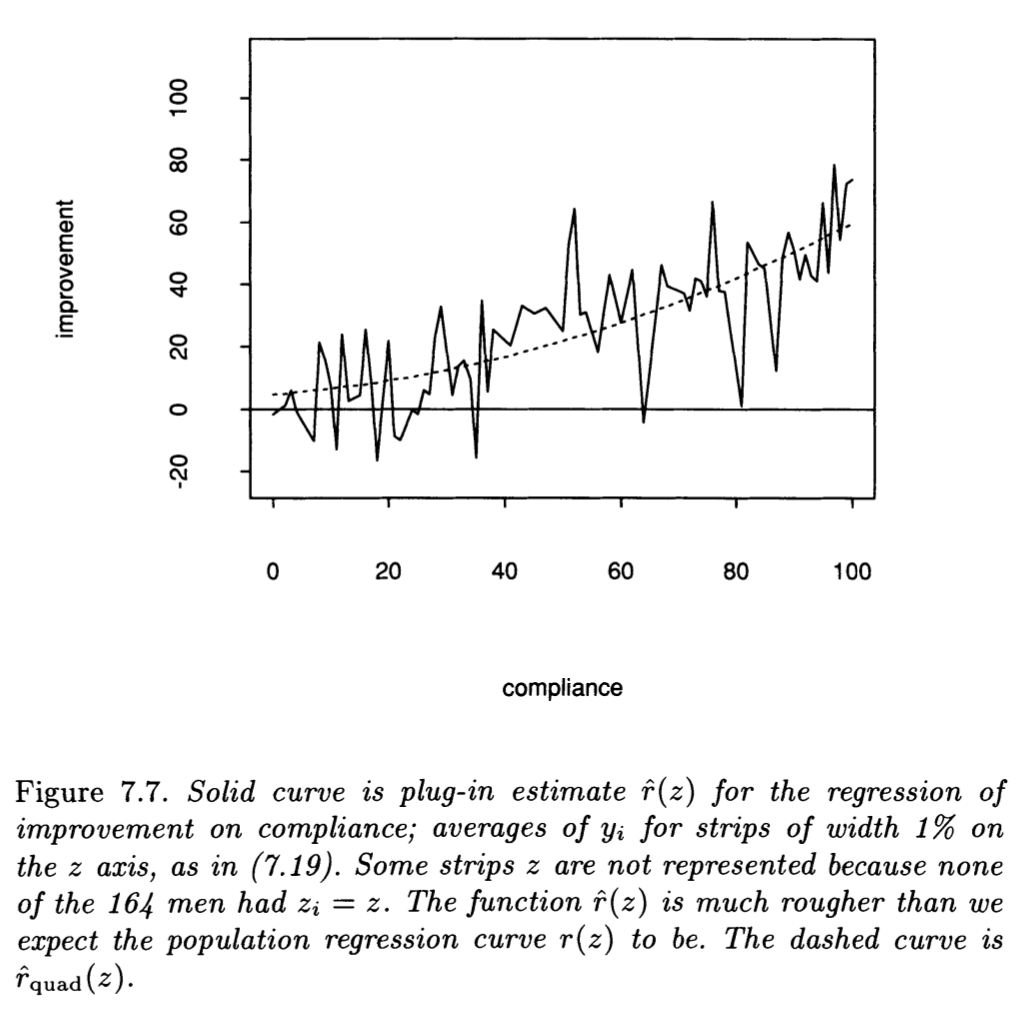
\includegraphics[width=0.9\linewidth]{6/f77.png}
\newline
\setcounter{figure}{7}

Впервые нашёлся пример, для которого метод подстановки работает не очень хорошо. Оценка регрессии $\hat r(z)$ гораздо грубее, чем мы хотели бы для оценки популяционной регрессии $r(z)$. Проблема в том, что внутри каждой полосы шириной в $1\%$ точек для адекватной оценки $r(z)$ недостаточно. Для некоторых полос шириной в $5\%$ точек внутри нет вообще. Мы можем увеличить ширину промежутка, скажем, до $10\%$ вместо $1\%$, но это не исправит проблему небольшого числа точек и, вероятно, проблема неустойчивости всё равно останется. На самом деле, имеется более элегантное и эффективное решение, которое основано на методе наименьших квадратов.

Использование метода начинается с предположения, что популяционная регрессионная функция, какая бы она не была, принадлежит семейству $\mathcal R$ гладких функций, индексированных вектором параметров $$\bm \beta = (\beta_0,\beta_1,\ldots,\beta_p)^\mathrm{T}$$. Для рассматриваемого примера мы ограничимся семейством квадратичных функций от $z$, скажем, $\mathcal R_\text{quad},$
\begin{equation}
  \mathcal R_\text{quad: \quad} r_{\bm \beta}(z) = \beta_0 + \beta_1 z + \beta_2 z^2,
\end{equation}
поэтому $\bm \beta = (\beta_0,\beta_1,\beta_2)^\mathrm{T}$. Далее мы обсудим выбор именно квадратичного семейства $\mathcal R_\text{quad},$ но на сейчас примем это как данное.

Читатель может представить себе выбор некоторого пробного значения $\bm \beta$, к примеру, $\bm \beta = (0,0.75,0.005)^\mathrm{T}$, и построение $r_\beta(z)$ на рисунке 7.5. Мы хотели бы, чтобы кривая $r_\beta(z)$ проходила близко к нашим данным $(z_i, y_i)$ в некотором общем смысле. Наиболее удобно для вычислений измерять близость кривой к данным с помощью суммы квадратов остатков (\textit{Residual Squared Error}),
\begin{equation}
  \rse(\bm \beta) = \sum_{i = 1}^n [y_i - r_{\bm \beta} (z_i)]^2.
\end{equation}
Сумма квадратов остатков получается опусканием вертикальных отрезков от каждой точки $(z_i, y_i)$ к кривой $r_{\bm \beta} (z_i)$, а затем суммированием квадратов их длин.

\textit{Метод наименьших квадратов}, созданные Гауссом и Лежандром в начале 19 века, выбирает среди кривых в $\mathcal R$ те, которые минимизируют $\rse$. Наилучший из них объявляется $r_{\hat {\bm \beta}}(z),$ где $\hat {\bm\beta}$ минимизирует $\rse(\bm \beta)$,
\begin{equation}
  \rse(\hat{\bm \beta}) = \min_{\bm \beta}{\rse(\bm \beta)}.
\end{equation}
 Кривая $\rquad(z)$ на рисунке 7.6 есть $r_{\hat{\bm \beta}}(z) = \hat \beta_0 + \hat \beta_1 z + \hat \beta_2 z^2,$ наилучшая квадратичная функция для наших данных.
 
 Лежандр и Гаусс обнаружили замечательную явную формулу для решения $\hat{\bm \beta}$ задачи наименьших квадратов. Пусть $\mathbf C$ есть матрица $164\times 3,$ $i$-я строка которой есть
 \begin{equation}
  \bm c_i = (1, z_i, z_i^2),
\end{equation}
и пусть $\mathbf y$ есть вектор из 164 значений $y_i.$ Тогда, используя стандартную матричную нотацию, имеем
\begin{equation}
  \hat{\bm \beta} = (\mathbf C^\mathrm{T} \mathbf{C})^{-1} \mathbf{C}^\mathrm{T} \mathbf y.
\end{equation}
Более  подробно мы рассмотрим эту формулу в главе 9. Для наших целей, связанных с применением бутстрепа, нам достаточно лишь знать про то, что набор данных из $n$ пар $\mathbf x = (\mathbf x_1, \mathbf x_2,\ldots, \mathbf x_n)$ приводит к получению квадратичной кривой $r_{\hat{\bm \beta}}(z)$ через отображение $\mathbf x \rightarrow r_{\hat{\bm \beta}}(z),$ которое описывается (7.23), (7.24) и (7.20).

Можно рассматривать $r_{\hat{\bm \beta}}(z)$ как сглаженную версию оценки по методу подстановки $\hat r(z)$. Предположим, что мы бы рассмотрели более широкий класс гладких функций $\mathcal R,$ к примеру, класс кубических функций $\mathcal R_\text{cubic}.$ В таком случае решение по методу наименьших квадратов $r_{{\hat{\bm\beta}}}(z)$ стало бы ближе к данным, однако оказалось бы более <<бугристым>>, чем квадратичное решение по методу наименьших квадратов. Если бы мы начали рассматривать полиномы всё большей степени, $r_{\hat{\bm \beta}}$ всё больше бы походил на оценку по методу подстановки $\hat r  (z)$. Выбор семейства квадратичных функций основан на нашем представлении о том, насколько гладкой должна быть оригинальная функция регрессии $r(z)$.
 Смотря на рисунок 7.7, мы явно видим, что $\rquad(z)$ гораздо более гладкая, чем $\hat r (z),$ однако в целом соответствует $\hat r (z)$ как функция от $z$.
 
Легко поверить, что настоящая функция регрессии $r(z)$ есть гладкая функция от $z$.  Сложнее поверить в то, что $r(z)$ является квадратичной от $z$ для всех значений $z$. Сглаживающая функция \textit{loess} является компромиссом между \textit{глобальными} предположениями о форме и чисто \textit{локальным} усреднением $\hat r(z)$.  

Для использования loess нужно указать число $\alpha$, которое равно части $n$ точек, используемых при построении кривой в каждой из точек. Кривая $\rloess (z)$ на рисунке 7.6 построена при выборе $\alpha = 0.3$. Для каждого из значений $z$ значение $\rloess (z)$ получается следующим образом:
\begin{enumerate}
	\item $n$ точек $\mathbf x_i = (z_i, y_i)$  упорядочиваются согласно $|z_i - z|,$ а ближайшие $\alpha \cdot n$ точек с наименьшим $|z_i - z|$, запоминаются. Назовём эти точки $\mathcal N(z)$.\footnote{при выборе $\alpha= 0.3, n=164$, алгоритм выбирает в $\mathcal N(z)$ 49 точек}
	\item Взвешенная линейная регрессия (с минимизацией наименьших квадратов) 
	\begin{equation}
  	\hat r_z(Z) = \hat \beta_{z,0} + \hat \beta_{z,1} Z
	\end{equation}
	производится для $\alpha \cdot n$ точек в $\mathcal N(z)$. [То есть коэффициенты $ \hat \beta_{z,0}$ и $\hat \beta_{z,1}$ выбираются как минимизирующие $\sum_{\mathbf x_j \in \mathcal N} w_{z,j} [y_j - (\beta_0 + \beta_1 z_j)]^2$, где веса $w_{z,j}$ есть положительные числа, зависящие от $|z_j - z|$. Взяв 
	\begin{equation}
  u_j = \frac{|z_j - z|}{\max_{\mathcal N (z)}|z_k - z|},
\end{equation}
веса $w_j$ выбираются равными $(1 - u_j^3)^3$.]

	\item В итоге, $\rloess (z)$ назначается равным числу $\hat r_z(Z)$ в точке $Z = z,$
\begin{equation}
  \rloess(z) = \hat r_z (Z=z).
\end{equation}
\end{enumerate}
~\\
\noindent
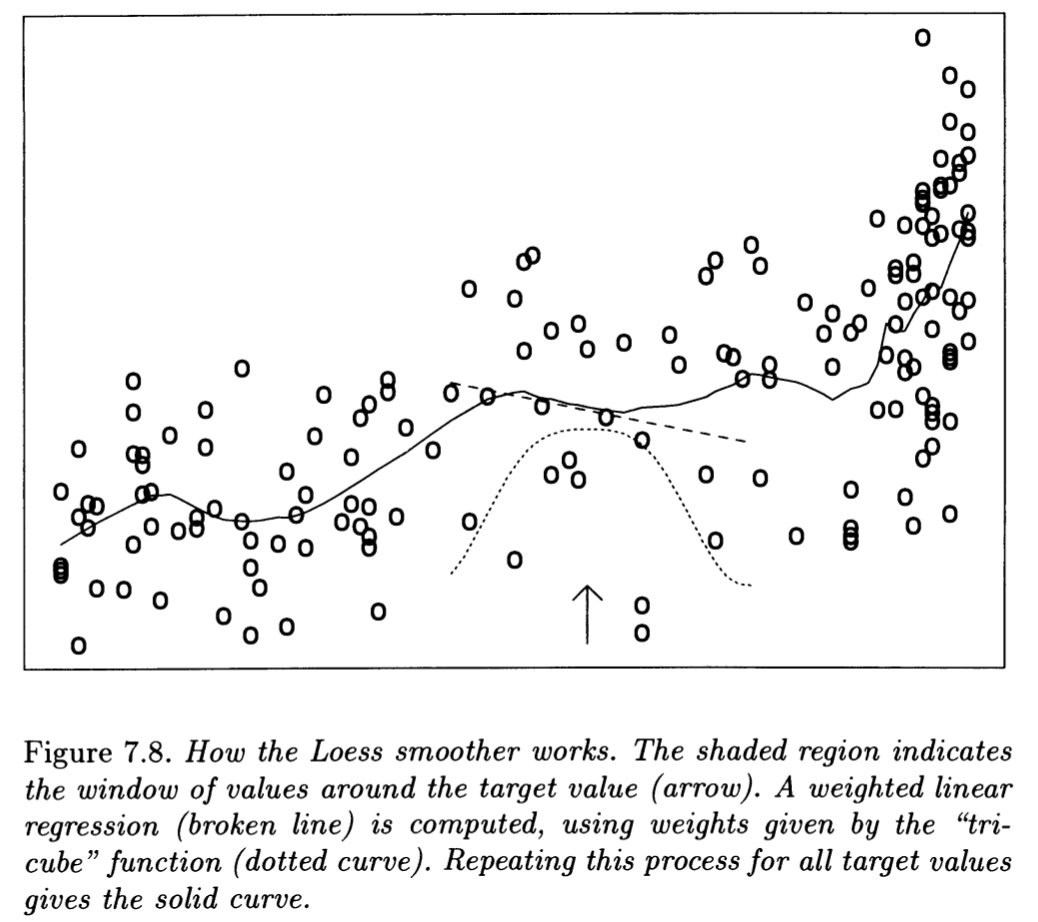
\includegraphics[width=0.9\linewidth]{6/f78.png}
\newline
\setcounter{figure}{8}

Компоненты loess сглаживания показаны на рисунке 7.8. В таблице 7.5 показано сравнение $\rquad(z)$ и $\rloess(z)$ в двух значениях, представляющих наибольший интерес, $z = 60\%$ и $z = 100\%$. Стандартные ошибки по бутстрепу даны для каждого из значений. Они были получены из $B = 50$ бутстреп репликаций алгоритма, показанного на рисунке 6.1.
\\~\\
\noindent
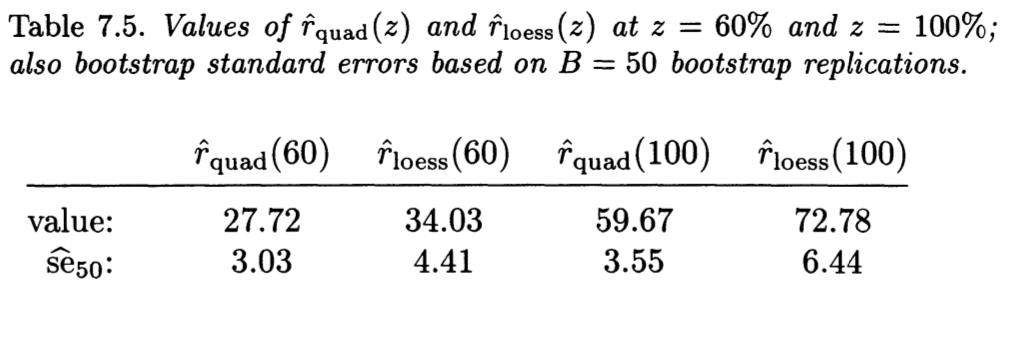
\includegraphics[width=0.9\linewidth]{6/t75.png}
\newline
\setcounter{table}{5}

В данном случае $\hat F$ есть распределение, дающее вероятность $1/164$ каждому из 164 наблюдений $\mathbf x_i = (z_i, y_i).$ Бутстреп набор есть $\mathbf x^* = (\mathbf x_1^*,\mathbf x_2^*, \ldots, \mathbf x_{164}^*),$ где каждый из $\mathbf x_i^* $ равен одному из 164 наблюдений с одинаковой вероятностью. Получив $\mathbf x^*,$ мы вычислили $\rquad^*(z)$ и $\rloess^*(z)$, квадратичную и loess кривые на основе $\mathbf x^*.$ В завершение мы вычислили значения $\rquad^*(60)$ и $\rloess^*(60)$, а также $\rquad^*(100)$ и $\rloess^*(100)$. $B = 50$ значений $\rquad^*(60)$ имеют стандартную ошибку $3.03$ и т.д., см. таблицу 7.5.

Посмотрев на результаты в таблице 7.5, можно сделать вывод о том, что оценка $\rloess(z)$ значительно менее точна, чем $\rquad(z).$	Это неудивительно, ведь $\rloess(z)$ строится на меньшем количестве данных (размер обусловлен $\alpha$), чем $\rquad(z)$. Неустойчивость $\rloess(z)$ очевидна по графикам на рисунке 7.9.
\\~\\
\noindent
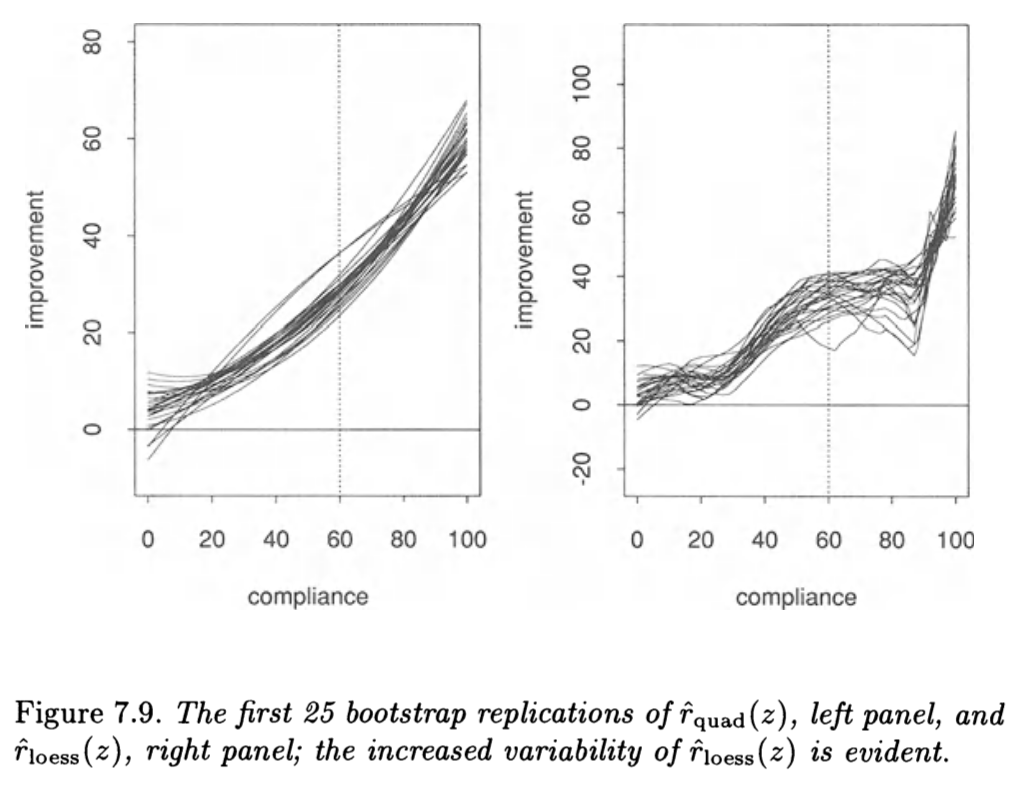
\includegraphics[width=0.9\linewidth]{6/f79.png}
\newline
\setcounter{figure}{9}

Полезно построить кривые бутстрепа, чтобы увидеть, сохраняются ли некоторые интересные особенности оригинальной кривой у кривых по бутстреп выборкам. Например, на рисунке 7.6 видим, что $\rloess(z)$ растёт гораздо быстрее с $z = 80\%$ до $z = 100\%$, чем с $z = 60\%$ до $z = 80\%$. Разность средних у углов наклона составляет
\begin{align}
	\thetahat &= \frac{\rloess(100) - \rloess(80)}{20} - \frac{\rloess(80) - \rloess(60)}{20}\nonumber \\
	&= \frac{672.78 - 37.50}{20} - \frac{32.50 - 34.03}{20} = 1.84.
\end{align}
  
Соответствующее число для $\rquad$ составляет лишь $0.17$. Большинство loess кривых показывают похожий быстрый рост примерно на $80\%$. Ни одно из бутстреп значений $\thetahat^*$ не было меньше нуля, минимум составил 0.23, большинство значений оказались больше единицы, см. рисунок 7.10.
\\~\\
\noindent
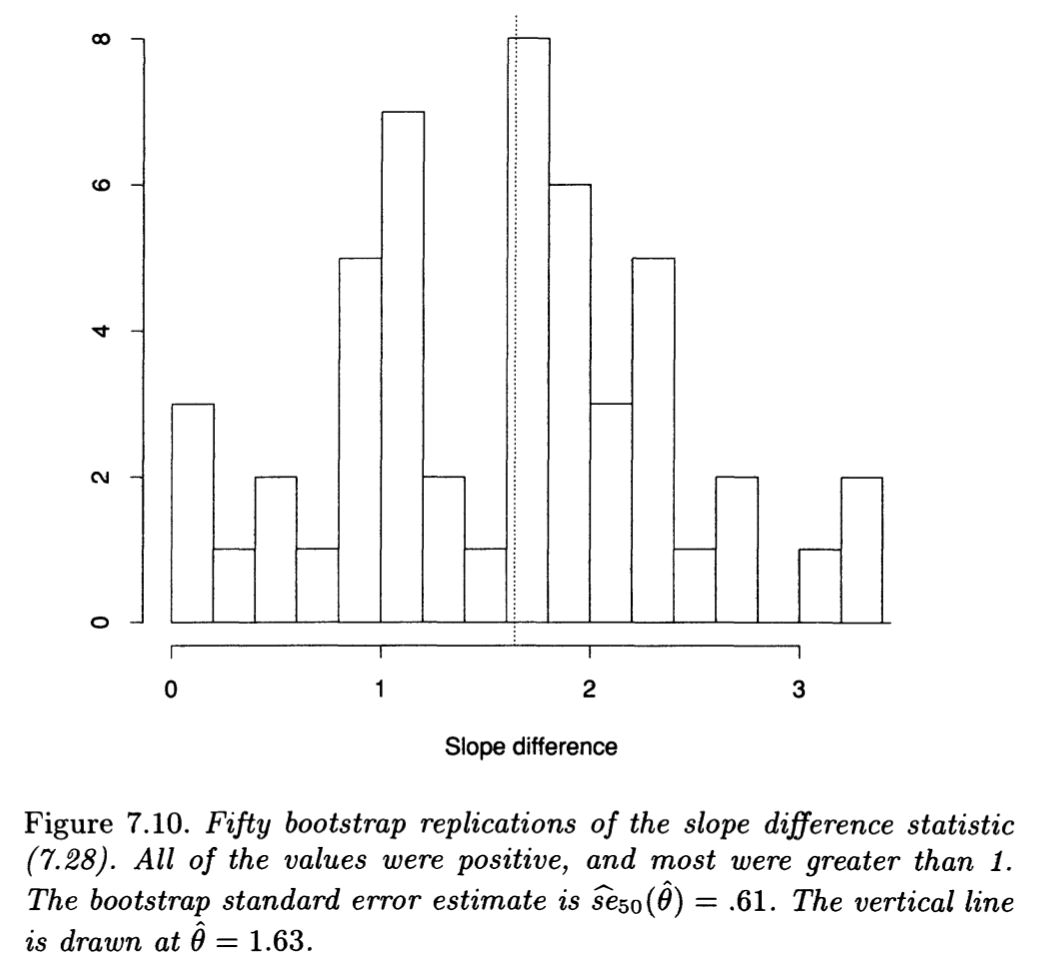
\includegraphics[width=0.9\linewidth]{6/f710.png}
\newline
\setcounter{figure}{10}
В такой момент мы можем законно опасаться того, что $\rquad(z)$ является \textit{слишком} гладкой оценкой оригинальной регрессионной функции $r(z)$. Если значение настоящей разности в углах наклона
\begin{equation}
  \theta = \frac{r(100) - r(80)}{20} - \frac{r(80) - r(60)}{20}
\end{equation}
и находится около $\thetahat = 1.59,$ то $r(z)$ будет выглядеть скорее как 
$\rloess(z)$, чем $\rquad(z)$ для $z$ между 60 и 100. Оценки, построенные на $\rloess(z)$ обычно отличаются высокой дисперсией, как в таблице 7.5, но в то же время имеют низкое смещение. Оба этих свойства происходят от локального характера алгоритма loess, который строит оценку $r(z)$ используя только элементы выборки в окрестности $z$.

Оценка $\thetahat = 1.59$, построенная на $\rloess$ имеет большую вариативность, $\seh_{50} = 0.61$, однако содержание рисунка 7.10 явно намекает на то, что настоящее значение $\theta$, каким бы оно ни было, больше, чем значение $\thetahat = 0.17,$ основанное на $\rquad.$ Мы рассмотрим эту проблему детальнее в главах 12--14 про бутстреп доверительные интервалы.

Таблица 7.5 намекает на то, что нам следует беспокоиться за оценки $\rquad(60)$ и $\rquad(100),$ которые могут быть значительно заниженными. Одним из возможных решений этой проблемы может быть выбор полиномиальных моделей более высокой размерности. Достаточно замысловатые теории построения моделей были предложены с целью определить, когда следует продолжать поиск модели в пространстве большей размерности, а когда следует остановиться. Мы глубже рассмотрим вопрос построения регрессионных моделей в главе 9, где данные примера 2 мы рассмотрим снова. Простые бутстреп оценки вариативности и неустойчивости, которые были освещены в данной главе, часто становятся полезным шагом в сторону понимания регрессионных моделей, в особенности нетрадиционных (таких как $\rloess(z)$).